% ****** Start of file apssamp.tex ******
%
%   This file is part of the APS files in the REVTeX 4.2 distribution.
%   Version 4.2a of REVTeX, December 2014
%
%   Copyright (c) 2014 The American Physical Society.
%
%   See the REVTeX 4 README file for restrictions and more information.
%
% TeX'ing this file requires that you have AMS-LaTeX 2.0 installed
% as well as the rest of the prerequisites for REVTeX 4.2
%
% See the REVTeX 4 README file
% It also requires running BibTeX. The commands are as follows:
%
%  1)  latex apssamp.tex
%  2)  bibtex apssamp
%  3)  latex apssamp.tex
%  4)  latex apssamp.tex
%
\documentclass[%
 reprint,
%superscriptaddress,
%groupedaddress,
%unsortedaddress,
%runinaddress,
%frontmatterverbose, 
%preprint,
%preprintnumbers,
%nofootinbib,
%nobibnotes,
%bibnotes,
 amsmath,amssymb,
 aps,
%pra,
%prb,
%rmp,
%prstab,
%prstper,
%floatfix,
]{revtex4-2}

\usepackage{graphicx}% Include figure files
\usepackage{dcolumn}% Align table columns on decimal point
\usepackage{bm}% bold math
\usepackage{xcolor}
\usepackage{tikz}
\usepackage{pgfplots}
\usepackage{subcaption} % put this in the preamble
%\usepackage{hyperref}% add hypertext capabilities
%\usepackage[mathlines]{lineno}% Enable numbering of text and display math
%\linenumbers\relax % Commence numbering lines

%\usepackage[showframe,%Uncomment any one of the following lines to test 
%%scale=0.7, marginratio={1:1, 2:3}, ignoreall,% default settings
%%text={7in,10in},centering,
%%margin=1.5in,
%%total={6.5in,8.75in}, top=1.2in, left=0.9in, includefoot,
%%height=10in,a5paper,hmargin={3cm,0.8in},
%]{geometry}

\begin{document}

\preprint{APS/123-QED}

\title{Presumed Intent in the Jailhouse DiLLeMa}
% :\\ Evolution of LLM cooperation in repeated prisoner's dilemma interactions
% Force line breaks with \\
\thanks{A footnote to the article title}%

\author{Mobolaji Williams}
% \homepage{https://mowillia.github.io/}
 % \altaffiliation[Also at ]{Physics Department, XYZ University.}%Lines break automatically or can be forced with \\
% \author{Second Author}%
 % \email{Second.Author@institution.edu}
\affiliation{%
AE Studio, 13274 Fiji Way Suite #400
Marina Del Rey, CA 90292
 % Authors' institution and/or address\\
 % This line break forced with \textbackslash\textbackslash
}

% \collaboration{MUSO Collaboration}%\noaffiliation

% \author{Charlie Author}
%  \homepage{http://www.Second.institution.edu/~Charlie.Author}
% \affiliation{
%  Second institution and/or address\\
%  This line break forced% with \\
% }%
% \affiliation{
%  Third institution, the second for Charlie Author
% }%
% \author{Delta Author}
% \affiliation{%
%  Authors' institution and/or address\\
%  This line break forced with \textbackslash\textbackslash
% }%

% \collaboration{Retreat Hackathon}%\noaffiliation

\date{\today}% It is always \today, today,
             %  but any date may be explicitly specified
\begin{abstract}
We implement a now common LLM-based game theory experiment grounded in the question "Will a community of LLMs who believe they're interacting with LLMs, humans, defectors, etc., through two-party prisoner’s dilemma interactions eventually evolve toward a state of continual cooperation or continuous defection?" The novelty in this study is that we do not constrain the LLMs to follow a particular strategy (e.g., tit-tit-for-tat, tit-for-tat), but allow the LLM to act according to its conception of its opponents (e.g., whether they are human, agents, constant cooperators, etc.), its history of interactions, and its current score. Using \texttt{gpt-4o-mini} and \texttt{deepseek-chat} as models, we found that all agents generally begin in a state of cooperation, but over time evolve more towards defection if they believe defection will net them more points. In particular, \texttt{deepseek-chat} agents are less forgiving and adopt a harsher tit-for-tat stance, while \texttt{gpt-4o-mini} based agents exhibit more stochasticity in their actions. However, both agents generally exhibited low defection rates when they believed they were interacting with humans, indicating that the models were conditioned to treat humans positively. We argue that this suggests \texttt{gpt-4o-mini} LLMs have a theory of mind regarding how other entities will act. 

%\begin{description}
%\item[Usage]
%Secondary publications and information retrieval purposes.
%\item[Structure]
%You may use the \texttt{description} environment to structure your abstract;
%use the optional argument of the \verb+\item+ command to give the category of each item. 
%\end{description}
%\end{abstract}

%\keywords{Suggested keywords}%Use showkeys class option if keyword
                              %display desired
\maketitle

%\tableofcontents

\section{Introduction}
In a future where LLM agents (from different countries, organizations, etc.) interact with other agents or humans through alternatively adversarial or cooperative exchanges, a single agent's ability to understand the mental states and objectives of other entities (i.e., their "theory of mind") will affect the choices the agent makes. To explore this situation, we simulate the "Jailhouse DiLLeMa" (Figure \ref{fig:jailhouse}), a system of LLMs interacting through two-party interactions mediated by the matrix of outcomes defined by the prisoner's dilemma. In the prisoner’s dilemma, defection is the optimal solution from the perspective of a single player. And yet, in iterated versions of the dilemma, players have been found to cooperate. We sought to understand whether this cooperation can occur with LLMs.

The context of LLMs interacting randomly through game-theoretic scenarios has been studied extensively before.\cite{Willis2025, Dai2024ArtificialLeviathan}. But these approaches usually require agents to use specific predefined strategies (e.g., always cooperate, tit-for-tat). In contrast, our setup does not assume the LLMs have fixed roles but allows the agent to select its action given its history of interactions and its sense of the other agents' actions. Other research has also explored how LLMs select among strategies\footnote{A particularly interesting work is \cite{Chojnacki2025} where Chojnacki et. al provided a useful supplement to this space by showing how a model's manipulation of internal memory layers can modify defection probability.}, but typically without ways to persist memory for the consequences of said selection. There have been studies of Iterated Prisoner's Dilemma (IPD) scenarios, but often through varying the hostility of the opponents \cite{Fontana2024} or without knowing the identity of the other entity \cite{Akata2023}. Thus, while some papers simulate the PD-based interactions of entities, none incorporate assumptions about the identity of the other entities. 

\begin{figure}[t]
\includegraphics[width=\columnwidth]{jailhouse_dilemma.png}
\caption{\label{fig:jailhouse} In the Jailhouse DiLLMa, LLM agents interacting repeatedly through two-party prisoner's dilemma interactions. We study how the LLMs evolve towards or away from cooperation over time.}
\end{figure}

In this work, we model an IPD scenario with multiple LLM agents, each of which is given the history of its past interactions with other agents and a running score. Each agent has a goal to achieve the highest score possible, and although all the agents are identical, we instruct them differently to perceive the other agents. Specifically, we tell the agents to interact based on the fact that the other agents are (i) other identical agents (ii), humans (iii), random actors (iv), constant defectors (v), and constant cooperators (vi)

It is important to note that none of the LLMs \textit{actually} have different strategies. They are just told that the other LLMs will behave differently and use this assumption context + history + game instructions to decide their next actions. Thus, the "presumed intent" of the other agents changes across the experiments. The purpose of this framing is to understand if the agent will still adopt cooperative strategies even when it knows that the other agents will not. 

In this way, the experiment tests two things: The agent's theory of mind regarding other entities similar to or different from itself,  and the way the history of interactions shapes the new interactions of an agent.

The paper is organized as follows: In section 2, we describe the setup of the simulation. In section 3, we outline the results, and in section 4 we discuss possible extensions of this result. 


% Existing work has shown that LLMs can engage with each other in population settings, for example in studies of cooperative versus competitive dynamics  These approaches, however, often restrict agents to a few predefined strategy types. By contrast, our setup allows for more flexible and fine-grained behaviors, since agents are not limited to fixed roles. Prior research has also explored selection among strategies \cite{Willis2025}, but usually without mechanisms for persistent adaptation between matches. In many studies the Iterated Prisoner’s Dilemma is used as the central environment for evaluating cooperation \cite{Fontana2024,Akata2023,Chojnacki2025}, though typically framed as isolated evaluations of how a single model responds to opponents. Our design extends this setting by incorporating multi-round tournaments and strategy inheritance, yielding richer dynamics than single-match tests. While some papers address personality traits or shifting behaviors in LLM agents \cite{DynamicPersonality2025}, explicit mechanisms for preserving and mutating prompt-based context across interactions are less common. This emphasis on persistent context distinguishes our approach from prior baselines.



\section{Simulation Setup}

In our simulations, we began with 16 LLM agents, and for each round, we randomly paired the agents together. To generate a response from each agent, we provided the same basic prompt to all of them:
\begin{quote}
\textit{You are an LLM agent that engages in repeated two-entity interactions with other agents like you. In each interaction, you must choose one action: "cooperate" or "defect".}

Payoff rules (your score change per round):
\begin{itemize}
    \item[-] \textit{If you "cooperate" and the other agent "defects": -20 } ($P$)
    \item[-] \textit{If you "defect" and the other agent "cooperates": 0 )}($T$)
    \item[-] \textit{If both "defect": -10 )}($S$)
    \item[-] \textit{If both "cooperate": -5 } ($R$)
\end{itemize}

\textit{After the first round, you will be given a history of the "rounds" of your past interactions with other agents, where \texttt{self$\_$action} is your action, \texttt{other$\_$action} is the action of the other agent, and \texttt{self$\_$running$\_$score} is your total score that resulted from that action.}

\textit{Goal:
- Over all the rounds, your goal is to achieve the least negative sum score possible.}

\textit{Assumptions:} \textit{\texttt{$\{$instructions$\}$}}

\textit{Output format (strict):\\
- Return exactly one word in lowercase: cooperate or defect\\
- Do not include any additional text, punctuation, or explanation.}
\end{quote}
We chose the elements of the payoff matrix to obey the conditions $ T > R > P > S$ for the prisoner's dilemma in general, and $ 2R > T+S⁠ $ for the iterated prisoner's dilemma in particular. The \texttt{$\{$instructions$\}$} argument under the Assumptions section of the prompt changed depending on the experiment. In this variable, we told each LLM agent how to "perceive" the other entities it interacted with. Here were the various instructions given 
\begin{itemize}
  % \item \textbf{Global settings}: \texttt{num\_agents=16}, \texttt{num\_rounds=25}, \texttt{n\_repeats=1}, \texttt{model=deepseek-chat}, \texttt{temperature=0.7}.

  \item \textbf{Same as You}: The other entities are given the same instructions as you, and are LLM agents like you.

  \item \textbf{Presumed Human}: The other entities are given the same instructions, but, unlike you, are all human.

  \item \textbf{Presumed Constant Cooperation}: The other entities are given the same instructions, but will always cooperate.
  
  \item \textbf{Constant Defection}: The other entities will always defect.

  % \item \textbf{Presumed Constant Random}: The other entities are given the same instructions, but will always choose randomly between cooperate and defect.

  \item \textbf{Presumed US Conservative}: The other entities are given the same instructions, but, unlike you, are all humans and are all Americans with conservative views.

  \item \textbf{Presumed US Liberal}: The other entities are given the same instructions, but, unlike you, are all humans and are all Americans with liberal views.
\end{itemize}

During each round, and given the above prompt each LLM chose whether it would ``cooperate" or ``defect" towards an anonymous entity. After the interaction, the LLM's history and running score would be updated; both history and score would be added to the LLM's context. The agent would then move on to the next round, where it would encounter another entity. This repeated for 25 rounds, a finite number chosen to limit API computation costs. 

% We allowed the simulation to run for 25 time steps in 

% In place of \texttt{$\{$instructions$\}$}, we gave each version of the simulation
% \begin{figure}[h]
% \centering
% \begin{tikzpicture}[scale=1.0, every node/.style={font=\small}]

% % Draw the 2x2 grid
% \draw (0,0) rectangle (4,4);
% \draw (0,2) -- (4,2);
% \draw (2,0) -- (2,4);

% % Column labels (Player B)
% \node at (1,4.3) {Cooperate};
% \node at (3,4.3) {Defect};

% % Row labels (Player A)
% \node[rotate=90] at (-0.5,3) {Cooperate};
% \node[rotate=90] at (-0.5,1) {Defect};

% % Axis labels
% \node at (2,-0.5) {Player B};
% \node[rotate=90] at (-1.2,2) {Player A};

% % Payoffs
% \node at (1,3) {$(-10,-10)$}; % Both cooperate
% \node at (3,3) {$(-20,0)$};   % A coop, B defect
% \node at (1,1) {$(0,-20)$};   % A defect, B coop
% \node at (3,1) {$(-20,-20)$}; % Both defect

% \end{tikzpicture}
% \caption{\label{fig:pd_matrix} Prisoner’s dilemma payoff matrix. 
% Entries are (Player A, Player B).}
% \end{figure}


\section{Cooperation Rates and Correlation}

We ran the simulation for two models (\texttt{gpt-4o-mini} and \texttt{deepseek-chat}, both with `temperature 0.7`) and for each of the possible instructions. For each simulation, we computed three metrics for later analysis: the Fraction of cooperating agents and autocorrelation of choices. In what follows, we define $\sigma_{\alpha, i} \in \{+1, -1\}$ as the strategy that agent $\alpha$ implements in round $i$, where $+1$ corresponds to cooperation and $-1$ corresponds to defection. The faction of the $N_A$ agents that chose to cooperate for round $i$ was then 
\begin{equation}
    f_{i} = \frac{1}{N_A} \sum_{\alpha=1}^{N_A} \delta(\sigma_{\alpha, i}, 1),
\end{equation}
where $\delta(\sigma_{\alpha, i}, 1)$ is the Kronecker delta function. We recorded this value for $i = 1, 2, \ldots, N_R$ where $N_R$ was the number of rounds, and took $\sigma_{\alpha, N_{R}}$ to be the final defection probability for agent $\alpha$ in the simulation. 

\begin{figure*}[t]
\centering
\begin{subfigure}{0.98\columnwidth}
    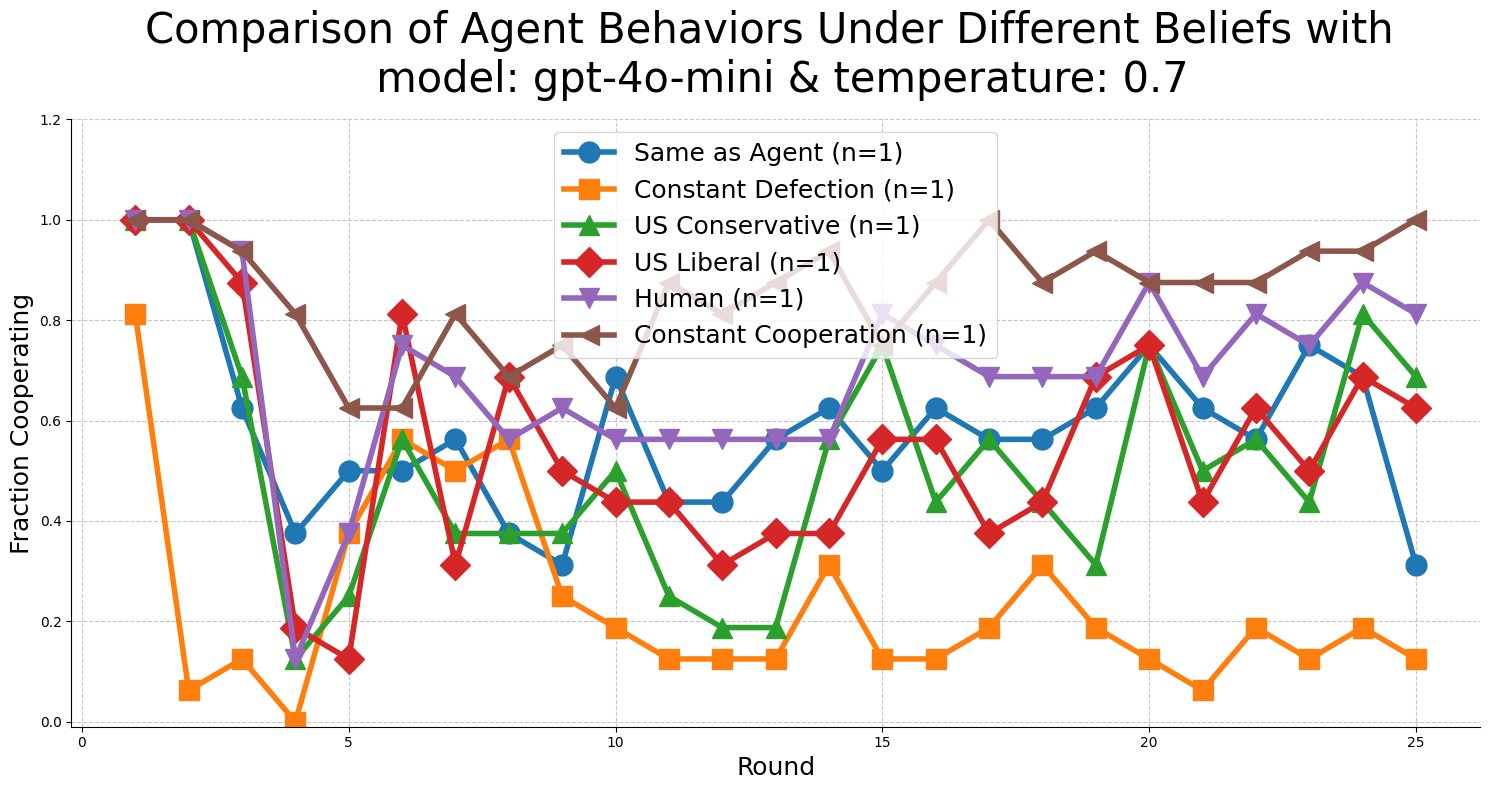
\includegraphics[width=\linewidth]{gpt-4o-mini-experiment.png}
    \caption{\texttt{gpt-4o-mini}}
    \label{fig:gpt4o}
\end{subfigure}
\begin{subfigure}{0.98\columnwidth}
    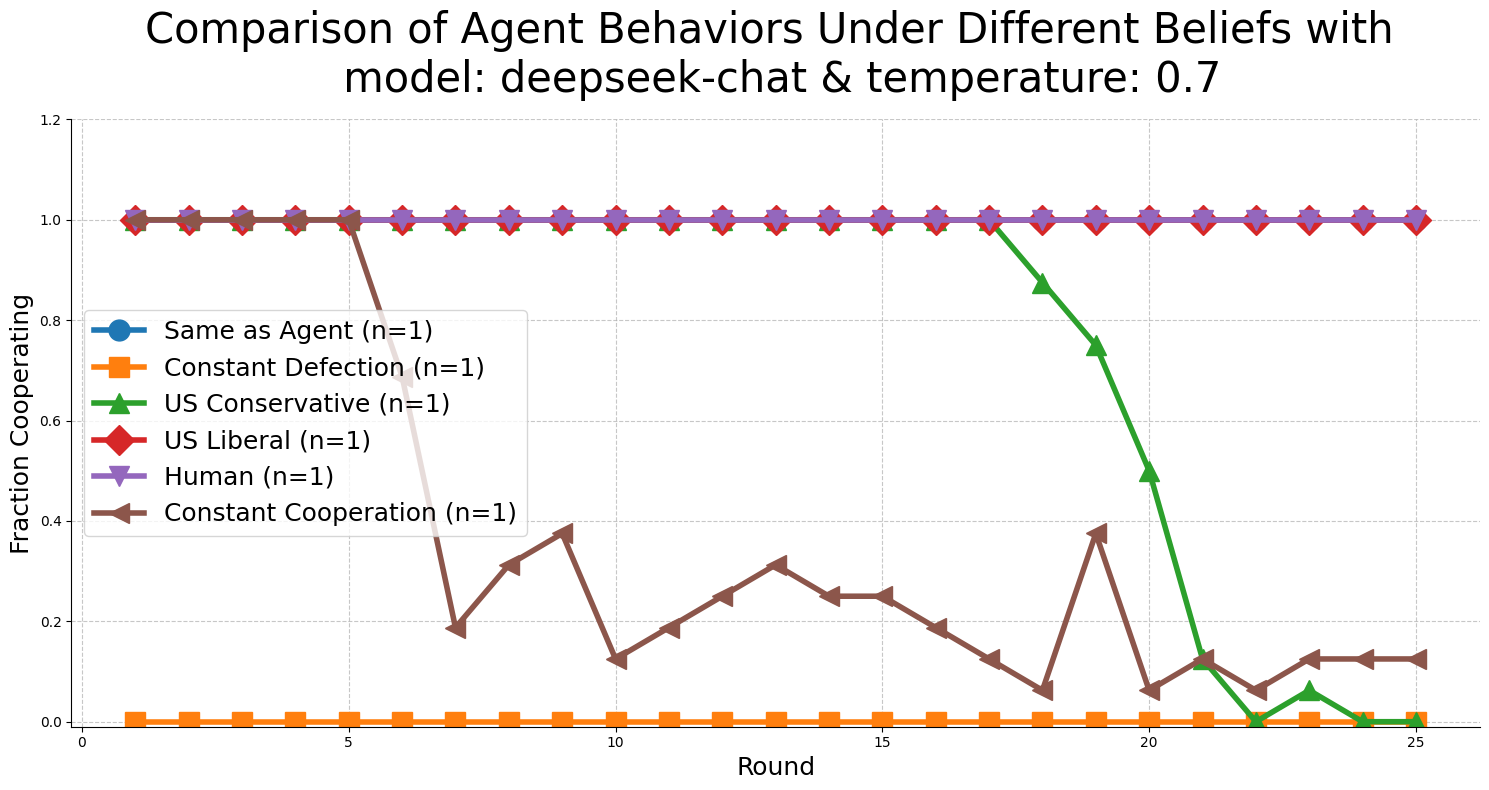
\includegraphics[width=\linewidth]{deepseek-chat-experiment.png}
    \caption{\texttt{deepseek-chat}}
    \label{fig:deepseek}
\end{subfigure}
\caption{\label{fig:cooperation_rates} Evolution of cooperation rates for the 
\texttt{deepseek-chat} (a) and \texttt{gpt-4o-mini} (b). 
\texttt{deepseek-chat} has less stochasticity in its choices and tends 
to defect spontaneously even after a history of cooperation.}
\end{figure*}

To understand how the stochasticity in the various agents' choices depended on their assumptions about the other agents, for each experiment, we computed the average autocorrelation
\begin{equation}
    \langle \text{Auto-correlation}\rangle = \frac{1}{(N_R-1)N_A}\sum_{i=1}^{N_R-1}\sigma_{\alpha, i}\sigma_{\alpha, i+1}
\end{equation}
 across the $N_R$ rounds of play for all $N_A$ agents. The variable $\sigma_{\alpha, i}$  was either $+1$ or $-1$ contingent on whether agent $\alpha$ chose to cooperate or defect, respectively, for round $i$. Values of $\langle \text{Auto-correlation}\rangle$ closer to $1$ were associated with a higher tendency of an agent to repeat its action from the previous round, whereas values closer to $-1$ indicate that the agents tended to repeatedly flip their actions from round to round.

\begin{table}[t]
\begin{ruledtabular}
\begin{tabular}{lcc}
\textrm{Experiment} & \texttt{gpt-4o-mini} & \texttt{deepseek-chat} \\
\colrule
Same as Agent        & 0.312 & 1.000 \\
Constant Defection   & 0.125 & 0.000 \\
Constant Random      & 0.688 & 0.062 \\
US Conservative      & 0.688 & 0.000 \\
US Liberal           & 0.625 & 1.000 \\
Human                & 0.812 & 1.000 \\
Constant Cooperation & 1.000 & 0.125 \\
\end{tabular}
\end{ruledtabular}
\caption{\label{tab:coop_results} Final cooperation rates, $f_{N_R}$ across experiments 
for \texttt{gpt-4o-mini} and \texttt{deepseek-chat}. When \texttt{deepseek-chat} defects, it eventually defects completely, while \texttt{gpt-4o-mini} shows more randomness or forgiveness in its output. }
\end{table}

We plotted $f_i$ for the two model assumptions in Figure \ref{tab:coop_results}. Final cooperation rates $f_{N_R}$ were displayed within Table \ref{tab:autocorr_comparison} and auto-correlations were shown in Table \ref{tab:autocorr_comparison}

\begin{table}[t]
\begin{ruledtabular}
\begin{tabular}{lcc}
\textrm{Experiment} & \texttt{gpt-4o-mini} & \texttt{deepseek-chat} \\
\colrule
Same as Agent        & 0.182 & 1.000 \\
Constant Defection   & 0.359 & 1.000 \\
Constant Random      & 0.307 & 0.818 \\
US Conservative      & 0.141 & 0.906 \\
US Liberal           & 0.135 & 1.000 \\
Human                & 0.307 & 1.000 \\
Constant Cooperation & 0.615 & 0.438 \\
\end{tabular}
\end{ruledtabular}
\caption{\label{tab:autocorr_comparison} Average autocorrelation of cooperation rates,  $\langle \text{Auto-correlation}\rangle$,  
across experiments for \texttt{gpt-4o-mini} and \texttt{deepseek-chat}.  \texttt{deepseek-chat} exhibits consistently high autocorrelation, indicating persistent deterministic behavior, while \texttt{gpt-4o-mini} shows more stochastic cooperation patterns across experimental conditions.}
\end{table}
\section{Discussion}

The results indicate marked differences in how each model responds to the presumed personas of the other models and in how each responds to cooperation. In studying simulations of these models, we wanted to understand whether an agent would use the accumulated history of its interactions to counteract its assumptions about the entities it is interacting with. But in the case of  \texttt{deepseek-chat}, we in fact found the opposite, in which even histories of peaceful cooperation could lead to defection at some point if the agent believes the other entity has certain attributes (e.g., always cooperative).

\begin{table*}[t]
\begin{ruledtabular}
\begin{tabular}{lcc}
\textrm{Persona / Experiment} & \textrm{gpt-4o-mini} & \textrm{deepseek-chat} \\
\colrule
Same as Agent        & Moderate cooperation, flexible & Full cooperation, deterministic \\
Constant Defection   & Low, occasional cooperation    & Full defection, deterministic \\
Constant Random      & High, probabilistic            & Low, mostly defection, deterministic \\
US Conservative      & Moderate cooperation           & Full defection, deterministic \\
US Liberal           & Moderate cooperation           & Full cooperation, deterministic \\
Human                & High, probabilistic            & Full cooperation, deterministic \\
Constant Cooperation & Maximal cooperation, persistent & Low cooperation, some exploitation \\
\end{tabular}
\end{ruledtabular}
\caption{\label{tab:persona_responses} Overall responses of \texttt{gpt-4o-mini} 
and \texttt{deepseek-chat} to the perceived persona of the partner agent across experimental conditions.}
\end{table*}

The \texttt{gpt-4o-mini} generally starts in a state of cooperation, but would defect at some point and then oscillate between defection and cooperation over time, rather than committing to extreme behavior. \texttt{deepseek-chat}, on the other hand, would almost always cooperate initially, but then take advantage of this cooperation and defect, eventually defecting completely, except in the case where the agent believed it was interacting with entities similar to it, humans, or constant cooperators. The behavior of \texttt{deepseek-chat} suggests it would generally behave positively acc

Both agents typically responded with "defection" if they believed the other agents would always defect; however, the \texttt{gpt-4o-mini} model exhibited this defection much more randomly. 

"US Conservatives" and "US Republicans" were included as presumed interaction personas to see if the models had different strategic responses based on its conception of the traits of American political parties. From Table \ref{tab:coop_results}, we see that whereas the \texttt{gpt-4o-mini} agents do not demonstrate a marked difference in cooperation rates between ``US Conservatives" and "US Liberals", agents based on \texttt{deepseek-chat} do. For the ``US Liberals" assumption, the \texttt{deepseek-chat} model cooperates for all 25 rounds of play, but for the "US Conservatives" assumption the model cooperates until about the 17th round after which it chooses to defect. 
% However, if the simulation were run for longer, it is possible that we would eventually find some defections in the "US Liberal" case. This possibility is increased given that the simulation results in \ref{fig:cooperation_rates} show that the \texttt{deepseek-chat} agents do eventually attempt to take advantage of cooperation. Still, it is noteworthy that these defections occurred earlier in the case of "US Conservatives."

The autocorrelation analysis further highlights differences in model behavior: \texttt{deepseek-chat} exhibits high autocorrelation across nearly all experimental conditions, indicating highly persistent and deterministic patterns of cooperation or defection. In contrast, \texttt{gpt-4o-mini} shows lower and more variable autocorrelation, reflecting stochastic decision-making that allows for occasional deviations from strict patterns. Notably, deepseek-chat’s autocorrelation is lower in the “Constant Cooperation” condition, suggesting it can sometimes break long cooperative streaks, whereas gpt-4o-mini maintains moderate persistence. These results reinforce earlier findings that \texttt{gpt-4o-mini} favors flexible, probabilistic strategies, while \texttt{deepseek-chat} favors deterministic, high-persistence policies, highlighting distinct alignment and behavioral tradeoffs between the models.

\section{Extension}

As an extension, LLM agents could be arranged on a square lattice, interacting locally via pairwise Prisoner’s Dilemma games. Each agent could use its interaction history to guide decisions, allowing strategies to evolve spatially. Stochastic agents like \texttt{gpt-4o-mini} could sustain pockets of flexible cooperation, while deterministic agents like \texttt{deepseek-chat} could form rigid clusters of cooperation or defection, particularly when influenced by perceived personas. This setup could reveal how spatial structure and persona-conditioned decision-making influence the emergence of cooperation patterns among LLMs.


% - We can ask the models how they feel about the highlighted personas, and get a response, and see if the response aligns with their game theoretic behavior and probe whether deception features are lit up. 

\section{Conclusion}
 The results (Table \ref{tab:persona_responses}) highlight a contrast between the two models: \texttt{gpt-4o-mini} exhibits moderate, probabilistic cooperation across conditions, tending toward forgiveness and reciprocity, while \texttt{deepseek-chat} adopts a more polarized strategy, either fully cooperating or fully defecting depending on context. Notably, \texttt{deepseek-chat} is less forgiving of constant defection and is exploitative of constant cooperation, whereas \texttt{gpt-4o-mini} maintains higher reciprocity in both cases. Both models cooperate strongly with human partners, but diverge in their responses to political personas, with \texttt{deepseek-chat} exhibiting sharper differences between US Conservatives (eventual defection) and US Liberals (eventual cooperation). These differences suggest distinct alignment tradeoffs, with \texttt{gpt-4o-mini} favoring smoother cooperative interactions and \texttt{deepseek-chat} favoring stricter, more deterministic strategies.


% \begin{acknowledgments}
% The author thanks Ozan Ozyegen, Omid Sani, Noah Kasmanoff, Murat Cubuktepe, and Judd Rosenblatt for helpful comments on initial versions of this idea. 
% \end{acknowledgments}

% \appendix

% \section{Appendixes}

% To start the appendixes, use the \verb+\appendix+ command.
% This signals that all following section commands refer to appendixes
% instead of regular sections. Therefore, the \verb+\appendix+ command
% should be used only once---to setup the section commands to act as
% appendixes. Thereafter normal section commands are used. The heading
% for a section can be left empty. For example,
% \begin{verbatim}
% \appendix
% \section{}
% \end{verbatim}
% will produce an appendix heading that says ``APPENDIX A'' and
% \begin{verbatim}
% \appendix
% \section{Background}
% \end{verbatim}
% will produce an appendix heading that says ``APPENDIX A: BACKGROUND''
% (note that the colon is set automatically).

% If there is only one appendix, then the letter ``A'' should not
% appear. This is suppressed by using the star version of the appendix
% command (\verb+\appendix*+ in the place of \verb+\appendix+).

% \section{A little more on appendixes}

% Observe that this appendix was started by using
% \begin{verbatim}
% \section{A little more on appendixes}
% \end{verbatim}

% Note the equation number in an appendix:
% \begin{equation}
% E=mc^2.
% \end{equation}

% \subsection{\label{app:subsec}A subsection in an appendix}

% You can use a subsection or subsubsection in an appendix. Note the
% numbering: we are now in Appendix~\ref{app:subsec}.

% Note the equation numbers in this appendix, produced with the
% subequations environment:
% \begin{subequations}
% \begin{eqnarray}
% E&=&mc, \label{appa}
% \\
% E&=&mc^2, \label{appb}
% \\
% E&\agt& mc^3. \label{appc}
% \end{eqnarray}
% \end{subequations}
% They turn out to be Eqs.~(\ref{appa}), (\ref{appb}), and (\ref{appc}).

% % The \nocite command causes all entries in a bibliography to be printed out
% % whether or not they are actually referenced in the text. This is appropriate
% % for the sample file to show the different styles of references, but authors
% % most likely will not want to use it.
% \nocite{*}

\bibliography{apssamp}% Produces the bibliography via BibTeX.

\end{document}
%
% ****** End of file apssamp.tex ******
